\section{Poblaciones versus Muestras}
\subsection{Datos: Estad\'{i}stica en Mundiales de F\'{u}tbol}

\subsubsection{}
Utilizando el total de goles, es  decir, los goles convertidos por ambos equipos en un partido, se construir\'{a}n tres tablas de frecuencia con un n\'{u}mero de clases igual a 5, 15 y 30. Para ello se utilizar� la librer�a \LaTeX \textit{xtable}. \\

\begin{table}[ht]
\centering
\caption*{Total de Goles - K = 5}
\begin{tabular}{crccc}
  \hline
 & Limites & Marca & Mediana & Frec. Absoluta \\ 
  \hline
  $K_{1}$ & [0, 2.4 ] & 1 & 1 & 354 \\
  $K_{2}$ & ( 2.4 , 4.8 ] & 3 & 3 & 274 \\
  $K_{3}$ & ( 4.8 , 7.2 ] & 5 & 5 & 131 \\
  $K_{4}$ & ( 7.2 , 9.6 ] & 8 & 8 & 21 \\
  $K_{4}$ & ( 9.6 , 12 ] & 11 & 11 & 5 \\
   \hline
\end{tabular}
\end{table}

\begin{table}[ht]
\centering
\caption*{Total de Goles - K = 15}
\begin{tabular}{crccc}
  \hline
 & Limites & Marca & Mediana & Frec. Absoluta \\ 
\hline
  $K_{1}$ & [0, 0.8 ] & 0 & 0 & 54 \\
  $K_{2}$ & ( 0.8 , 1.6 ] & 1 & 1 & 149 \\
  $K_{3}$ & ( 1.6 , 2.4 ] & 2 & 2 & 151 \\
  $K_{4}$ & ( 2.4 , 3.2 ] & 3 & 3 & 163 \\
  $K_{5}$ & ( 3.2 , 4 ] & 4 & 4 & 111 \\
  $K_{6}$ & ( 4 , 4.8 ] & NA & NA & 0 \\
  $K_{7}$ & ( 4.8 , 5.6 ] & 5 & 5 & 74 \\
  $K_{8}$ & ( 5.6 , 6.4 ] & 6 & 6 & 30 \\
  $K_{9}$ & ( 6.4 , 7.2 ] & 7 & 7 & 27 \\
  $K_{10}$ & ( 7.2 , 8 ] & 8 & 8 & 12 \\
  $K_{11}$ & ( 8 , 8.8 ] & NA & NA & 0 \\                
  $K_{12}$ & ( 8.8 , 9.6 ] & 9 & 9 & 9 \\
  $K_{13}$ & ( 9.6 , 10.4 ] & 10 & 10 & 1 \\
  $K_{14}$ & ( 10.4 , 11.2 ] & 11 & 11& 3 \\
  $K_{15}$ & ( 11.2 , 12 ] & 12 & 12 & 1 \\
   \hline
\end{tabular}
\end{table}

\begin{table}[ht]
\centering
\caption*{Total de Goles - K = 30}
\begin{tabular}{crccc}
  \hline
 & Limites & Marca & Mediana & Frec. Absoluta \\ 
\hline
  $K_{1}$ & [0, 0.4 ] & 0 & 0 & 54 \\ 
  $K_{2}$ & ( 0.4 , 0.8 ] & NA & NA & 0 \\ 
  $K_{3}$ & ( 0.8 , 1.2 ] & 1 & 1 & 149 \\ 
  $K_{4}$ & ( 1.2 , 1.6 ] & NA & NA & 0 \\ 
  $K_{5}$ & ( 1.6 , 2 ] & 2 & 2 & 151 \\ 
  $K_{6}$ & ( 2 , 2.4 ] & NA & NA & 0 \\ 
  $K_{7}$ & ( 2.4 , 2.8 ] & NA & NA & 0 \\ 
  $K_{8}$ & ( 2.8 , 3.2 ] & 3 & 3 & 163 \\ 
  $K_{9}$ & ( 3.2 , 3.6 ] & NA & NA & 0 \\ 
  $K_{10}$ & ( 3.6 , 4 ] & 4 & 4 & 111 \\ 
  $K_{11}$ & ( 4 , 4.4 ] & NA & NA & 0 \\ 
  $K_{12}$ & ( 4.4 , 4.8 ] & NA & NA & 0 \\ 
  $K_{13}$ &( 4.8 , 5.2 ] & 5 & 5 & 74 \\ 
  $K_{14}$ & ( 5.2 , 5.6 ] & NA & NA & 0 \\ 
  $K_{15}$ & ( 5.6 , 6 ] & 6 & 6 & 30 \\ 
  $K_{16}$ & ( 6 , 6.4 ] & NA & NA & 0 \\ 
  $K_{17}$ & ( 6.4 , 6.8 ] & NA & NA & 0 \\ 
  $K_{18}$ & ( 6.8 , 7.2 ] & 7 & 7 & 27 \\ 
  $K_{19}$ & ( 7.2 , 7.6 ] & NA & NA & 0 \\ 
  $K_{20}$ & ( 7.6 , 8 ] & 8 & 8 & 12 \\ 
  $K_{21}$ & ( 8 , 8.4 ] & NA & NA & 0 \\ 
  $K_{22}$ & ( 8.4 , 8.8 ] & NA & NA & 0 \\ 
  $K_{23}$ & ( 8.8 , 9.2 ] & 9 & 9 & 9 \\ 
  $K_{24}$ & ( 9.2 , 9.6 ] & NA & NA & 0 \\ 
  $K_{25}$ & ( 9.6 , 10 ] & 10 & 10 & 1 \\ 
  $K_{26}$ & ( 10 , 10.4 ] & NA & NA & 0 \\ 
  $K_{27}$ & ( 10.4 , 10.8 ] & NA & NA & 0 \\ 
  $K_{28}$ & ( 10.8 , 11.2 ] & 11 & 11 & 3 \\ 
  $K_{29}$ & ( 11.2 , 11.6 ] & NA & NA & 0 \\ 
  $K_{30}$ & ( 11.6 , 12 ] & 12 & 12 & 1 \\ 
   \hline
\end{tabular}
\end{table}

Se puede observar en todos los casos que los datos est\'{a}n fuertemente concentrados en las primeras clases, es decir, la mayor\'{i}a de los partidos finalizaron con 0, 1, 2 o 3 goles. Adem\'{a}, encontramos valores NA y frecuencias 0 en varios de las clases debido a que no existen goles con n\'{u}meros no naturales, por ejemplo, es absurdo hablar de 1.4 goles. \\
Finalmente, podemos concluir que de nuestra muestra de 785 partidos disputados, la cantidad de goles se encuentra generalmente entre los 0 y los 3 goles anotados. \\

\subsubsection{}
Se construir\'{a}n 4 histogramas con n\'{u}mero de clases iguales a 5, 10, 30, y 100 que mostrar\'{a} la distribuci\'{o}n de frecuencias para la variable en estudio. Esto se realiz\'{o} utilizando al funci\'{o} \verb+hist+ de R. \\

\begin{center}
   N�mero de Clases: 5 \\
  	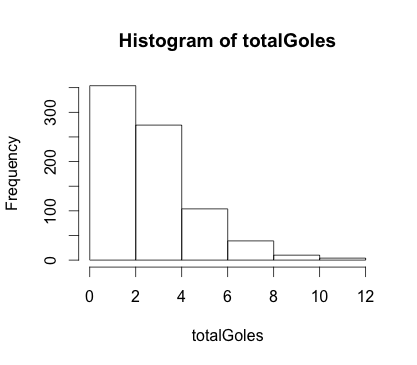
\includegraphics[width=0.9\textwidth]{./imagenes/hist1} \\
   N�mero de Clases: 10 \\ 
	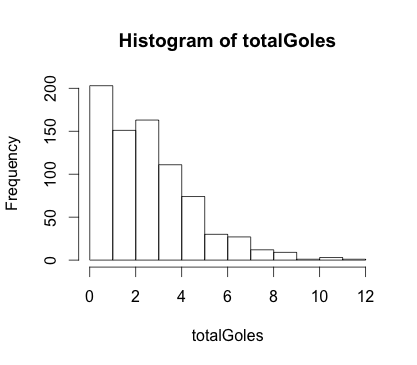
\includegraphics[width=0.9\textwidth]{./imagenes/hist2} \\
   N�mero de Clases: 30 \\
     	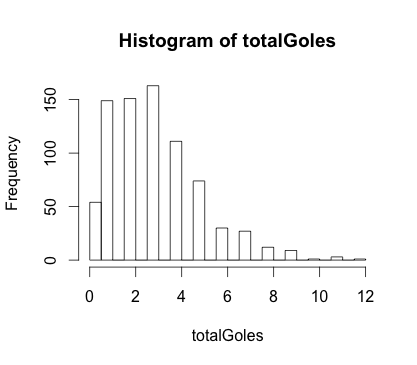
\includegraphics[width=0.9\textwidth]{./imagenes/hist3} \\
   N�mero de Clases: 100 \\ 
     	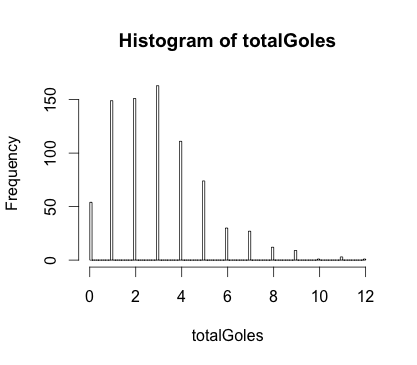
\includegraphics[width=0.9\textwidth]{./imagenes/hist4} \\
\end{center}

As\'{i} como nos fue posible observar mediante las tablas de la subsecci\'{o}n anterior, la distribuci\'{o}n de los goles, independiente de la cantidad de clases, est\'{a} centrada en el comienzo del histograma. Adem\'{a}s, notamos del primer histograma, que la mayor\'{i}a de los goles se centran en las clases que van entre los valores 0 y 3, pero a medida que aumentamos el n\'{u}mero de clases, es f\'{a}cil apreciar que la moda est\'{a} en los 3 goles. Nuevamente, notamos frecuencia 0 en las clases que s\'{o}lo contienen valores no enteros.\\

\subsubsection{}
Para esta \'{u}ltima subsecci�n, realizaremos los histogramas y divisiones de clases utilizando la regla de Sturges y utilizando muestras en vez del total de nuestra poblaci\'{o}n de datos, la cual ir\'{a} variando seg\'{u}n la siguiente instrucci\'{o}n: entre 10 y 100 de 10 en 10; luego entre 100 y 700 de 100 en 100. Para esta ocaci\'{o}n, utilizaremos el comando \verb+sample+ para conseguir una muestra aleatoria de nuestra poblaci\'{o}n y \verb+hist+ para construir histogramas. Por simplicidad, se mostrar\'{a}n s\'{o}lo 5 de los 16 histogramas, de cualquier forma, los dem\'{a}s se encontrar\'{a}n en la secci\'{o}n de anexos.\\

\begin{center}
  Tama\~{n}o muestral: 10 \\ 
  	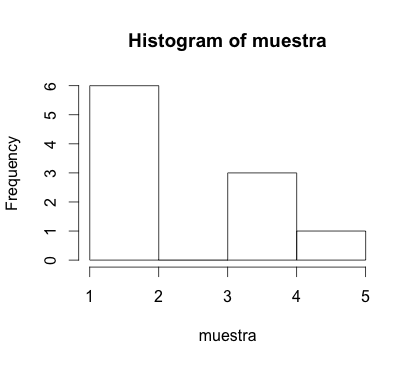
\includegraphics[width=0.9\textwidth]{./imagenes/histc1} \\
  Tama\~{n}o muestral: 50 \\ 
	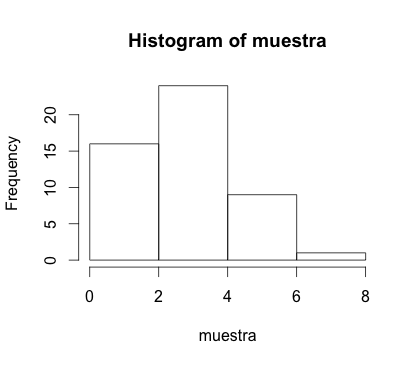
\includegraphics[width=0.9\textwidth]{./imagenes/histc5} \\
  Tama\~{n}o muestral: 100 \\ 
     	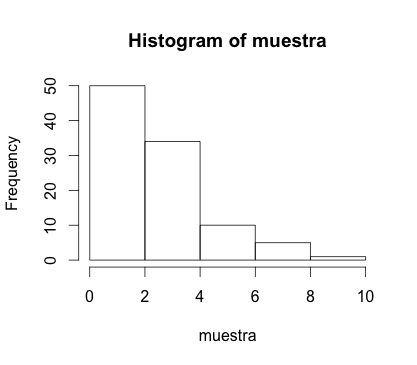
\includegraphics[width=0.9\textwidth]{./imagenes/histc10} \\
  Tama\~{n}o muestral: 300 \\ 
     	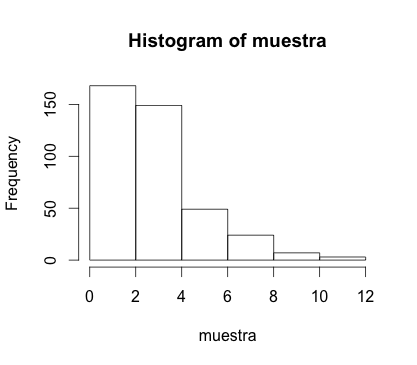
\includegraphics[width=0.9\textwidth]{./imagenes/histc13} \\
  Tama\~{n}o muestral: 700 \\ 
     	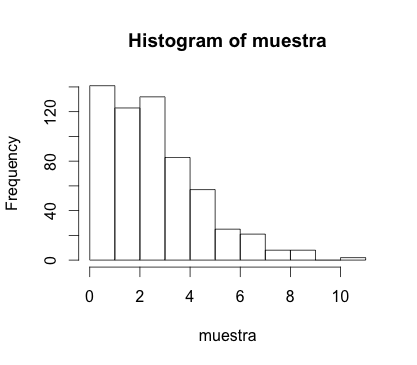
\includegraphics[width=0.9\textwidth]{./imagenes/histc15} \\	
\end{center}

Resulta sencillo concluir que los datos siguen centralizados en los primeros valores del histograma, a pesar de que la muestra es aleatoria. Por otra parte, notemos que los datos sobre 6 van apareciendo a medida que aumentamos el tama\~{o} de nuestra muestra, esto debido a que la cantidad de estos datos es bastante peque\~{n}a y la probabilidad de que aparezcan es tambi\'{e}n lo es.



\subsection{Medidas de Tendencia y Dispersi\'{o}n}

\subsubsection{}
Para nuestra variable de estudio, calcularemos la media, moda, mediana y varianza. 

\begin{table}[ht]
\centering
\begin{tabular}{cc}
  \hline
  Media & 3 \\ 
  Moda & 3 \\ 
  Mediana & 3 \\ 
  Varianza & 4.193878 \\
   \hline
\end{tabular}
\end{table}

\subsubsection{}
Se realizar\'{a} la confecci\'{o}n de un boxplot para nuestra variable Total de Goles utilizando el comando \verb+boxplot+ de R:

\begin{center}
   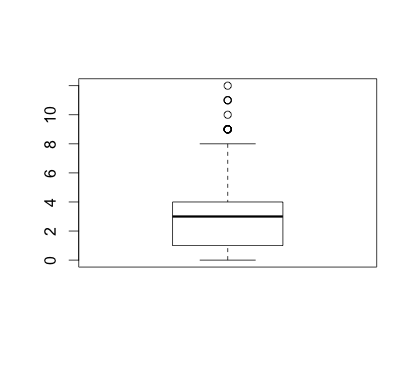
\includegraphics[width=0.9\textwidth]{./imagenes/boxplot}
\end{center}

Se puede observar la existencia de outliers, estos van desde los 8 (sin considerar este valor) hasta los 12 goles por partido. A pesar de la existencia de outliers, y como un buen conocedor de este deporte sabr\'{a}, una cantidad mayor a 8 goles por partido es rara vez apreciada, nuestra media no se ve afecta a ello, situaci\'{o}n que en pocas ocasiones sucede. Al contrario de los valores de media y mediana, la varianza si se ve afecta a estos outliers, por lo cual el valor de 4.193878 lo confirma. Gracias a estos valores, podemos afirmar que los partidos de mundiales la mayor\'{i} de los partidos jugados presenta una cantidad de 3 goles en total, de los cuales un equipo siempre saldr\'{a} victorioso.